\PassOptionsToPackage{unicode=true}{hyperref} % options for packages loaded elsewhere
\PassOptionsToPackage{hyphens}{url}
%
\documentclass[]{article}
\usepackage{lmodern}
\usepackage{amssymb,amsmath}
\usepackage{ifxetex,ifluatex}
\usepackage{fixltx2e} % provides \textsubscript
\ifnum 0\ifxetex 1\fi\ifluatex 1\fi=0 % if pdftex
  \usepackage[T1]{fontenc}
  \usepackage[utf8]{inputenc}
  \usepackage{textcomp} % provides euro and other symbols
\else % if luatex or xelatex
  \usepackage{unicode-math}
  \defaultfontfeatures{Ligatures=TeX,Scale=MatchLowercase}
\fi
% use upquote if available, for straight quotes in verbatim environments
\IfFileExists{upquote.sty}{\usepackage{upquote}}{}
% use microtype if available
\IfFileExists{microtype.sty}{%
\usepackage[]{microtype}
\UseMicrotypeSet[protrusion]{basicmath} % disable protrusion for tt fonts
}{}
\IfFileExists{parskip.sty}{%
\usepackage{parskip}
}{% else
\setlength{\parindent}{0pt}
\setlength{\parskip}{6pt plus 2pt minus 1pt}
}
\usepackage{hyperref}
\hypersetup{
            pdftitle={Problem set 2},
            pdfauthor={Juntong Lin},
            pdfborder={0 0 0},
            breaklinks=true}
\urlstyle{same}  % don't use monospace font for urls
\usepackage[margin=1in]{geometry}
\usepackage{graphicx,grffile}
\makeatletter
\def\maxwidth{\ifdim\Gin@nat@width>\linewidth\linewidth\else\Gin@nat@width\fi}
\def\maxheight{\ifdim\Gin@nat@height>\textheight\textheight\else\Gin@nat@height\fi}
\makeatother
% Scale images if necessary, so that they will not overflow the page
% margins by default, and it is still possible to overwrite the defaults
% using explicit options in \includegraphics[width, height, ...]{}
\setkeys{Gin}{width=\maxwidth,height=\maxheight,keepaspectratio}
\setlength{\emergencystretch}{3em}  % prevent overfull lines
\providecommand{\tightlist}{%
  \setlength{\itemsep}{0pt}\setlength{\parskip}{0pt}}
\setcounter{secnumdepth}{0}
% Redefines (sub)paragraphs to behave more like sections
\ifx\paragraph\undefined\else
\let\oldparagraph\paragraph
\renewcommand{\paragraph}[1]{\oldparagraph{#1}\mbox{}}
\fi
\ifx\subparagraph\undefined\else
\let\oldsubparagraph\subparagraph
\renewcommand{\subparagraph}[1]{\oldsubparagraph{#1}\mbox{}}
\fi

% set default figure placement to htbp
\makeatletter
\def\fps@figure{htbp}
\makeatother


\title{Problem set 2}
\author{Juntong Lin}
\date{2020/10/19}

\begin{document}
\maketitle

\begin{verbatim}
## -- Attaching packages ---------------------------------------------------------------- tidyverse 1.3.0 --
\end{verbatim}

\begin{verbatim}
## v ggplot2 3.2.1     v purrr   0.3.3
## v tibble  2.1.3     v dplyr   0.8.3
## v tidyr   1.0.0     v stringr 1.4.0
## v readr   1.3.1     v forcats 0.4.0
\end{verbatim}

\begin{verbatim}
## -- Conflicts ------------------------------------------------------------------- tidyverse_conflicts() --
## x dplyr::filter() masks stats::filter()
## x dplyr::lag()    masks stats::lag()
\end{verbatim}

\begin{verbatim}
## here() starts at /Users/apple/Desktop/problem-set-2
\end{verbatim}

\hypertarget{juntong-lin}{%
\section{Juntong Lin}\label{juntong-lin}}

\hypertarget{section}{%
\section{2020/10/19}\label{section}}

\hypertarget{abstract}{%
\subsection{Abstract}\label{abstract}}

This study is mainly to explore the relationship between people's
feelings of life and their individual income, and look out at which
level of income will have a significant impact. I also choose the
marital status, house owning or renting, and religion as the other
affecting variables on life feelings. A linear model is chosen for this
study. As a result, I find out individual income is a signifacnt factor,
however, the increase of feelings life is not that obvious in the first
four levels of income.

\hypertarget{introduction}{%
\subsection{Introduction}\label{introduction}}

In recent years, people are having more and more preasures, and it's
hard to have a satisfied life. After looking at this dataset, I'm
interested in the feelings of life of people, and would like to find out
some variables would have significant relation with it. Therefore, in
this study, I choose several varibles in common views that will affect
the feeligs of life. Since there are different levels in each variable,
when coding, I would set a base level for each of them. Also, as my main
focus is on individual income, I would study all the levels of income
and find out their relationship and significance. After that, I would
summary each level of income and code the regression of them. The result
of relationship of each variable may be easy to guess, but different
levels within each variables would have different significance.

\hypertarget{data}{%
\subsection{Data}\label{data}}

\begin{verbatim}
## Parsed with column specification:
## cols(
##   .default = col_character(),
##   caseid = col_double(),
##   age = col_double(),
##   age_first_child = col_double(),
##   age_youngest_child_under_6 = col_double(),
##   total_children = col_double(),
##   age_start_relationship = col_double(),
##   age_at_first_marriage = col_double(),
##   age_at_first_birth = col_double(),
##   distance_between_houses = col_double(),
##   age_youngest_child_returned_work = col_double(),
##   feelings_life = col_double(),
##   hh_size = col_double(),
##   number_total_children_intention = col_double(),
##   number_marriages = col_double(),
##   fin_supp_child_supp = col_double(),
##   fin_supp_child_exp = col_double(),
##   fin_supp_lump = col_double(),
##   fin_supp_other = col_double(),
##   is_male = col_double(),
##   main_activity = col_logical()
##   # ... with 1 more columns
## )
\end{verbatim}

\begin{verbatim}
## See spec(...) for full column specifications.
\end{verbatim}

feelings\_life, marital\_status, own\_rent, religion\_has\_affiliation,
and income\_respondent are the dat I decided to choose. I chose them
because they are some common views of happiness of life. Also, I decided
to remove the NAs in the data. There were 471 out of 20602 datas
contains NA, so removing them does not change the sample by much.

\hypertarget{model}{%
\subsection{Model}\label{model}}

I choose the linear model to study my hypothesis. I choose this model
because it is the most clear and simlified, since the variables are all
substring and have different levels. This will make it easier to set a
base model and study each level's significance.

\[Feelings\_life = a + b_1*marital\_status+ b2 *own\_rent + b3*religion\_has\_affiliation +b4*income\_respondent\]

\hypertarget{results}{%
\subsection{Results}\label{results}}

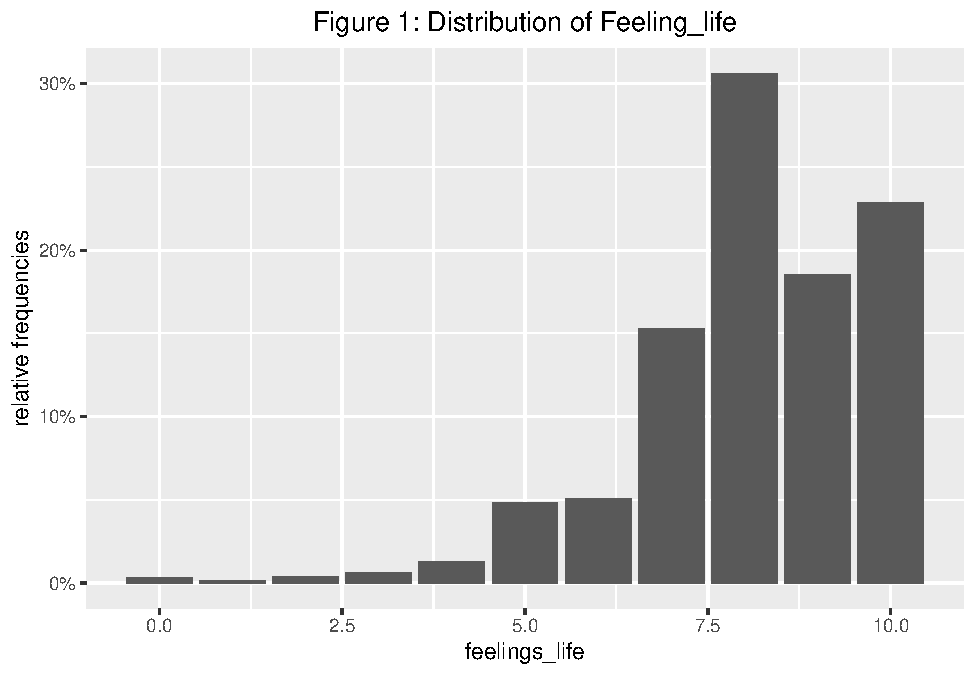
\includegraphics{ProblemSet2-template_files/figure-latex/unnamed-chunk-3-1.pdf}
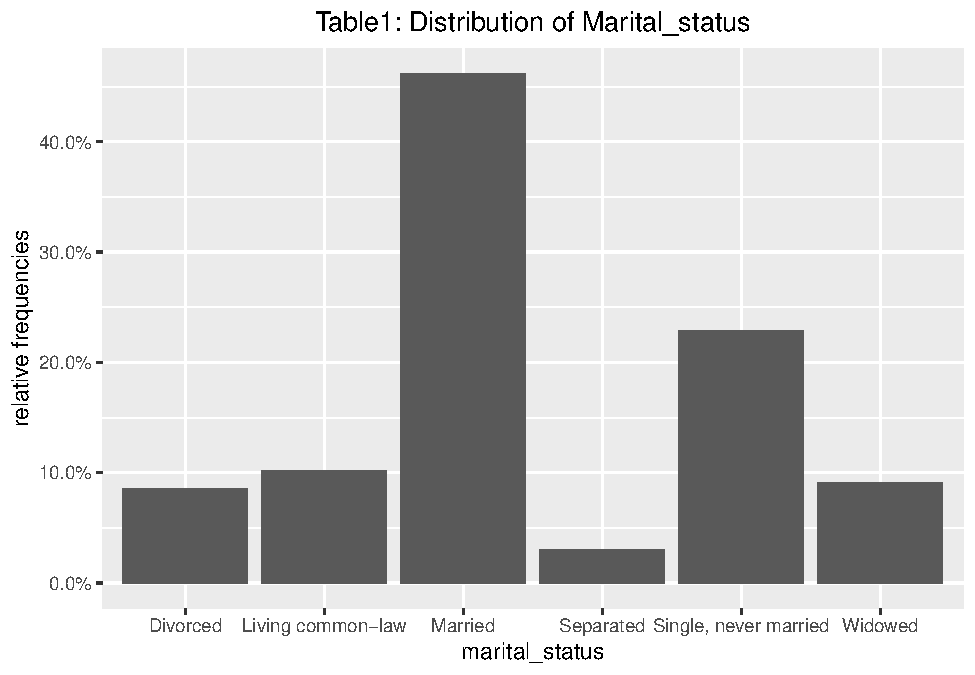
\includegraphics{ProblemSet2-template_files/figure-latex/unnamed-chunk-3-2.pdf}
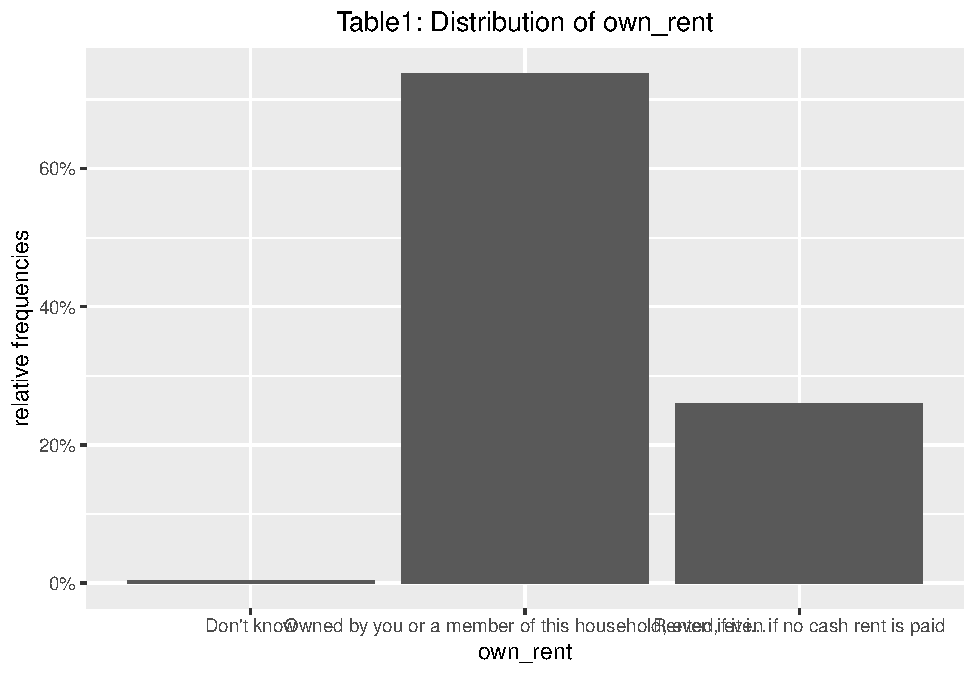
\includegraphics{ProblemSet2-template_files/figure-latex/unnamed-chunk-3-3.pdf}
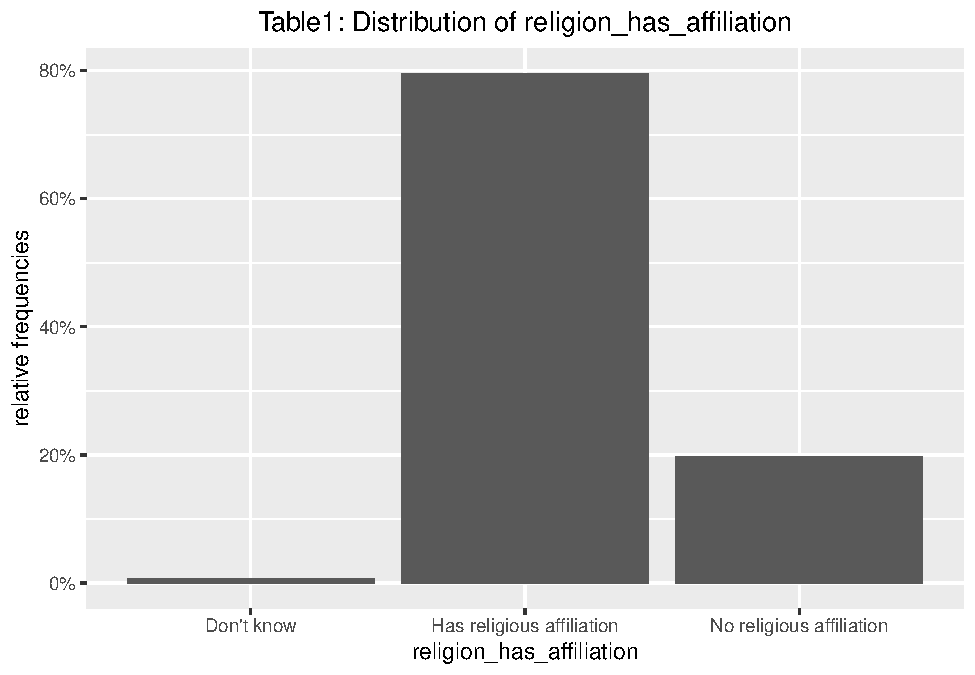
\includegraphics{ProblemSet2-template_files/figure-latex/unnamed-chunk-3-4.pdf}
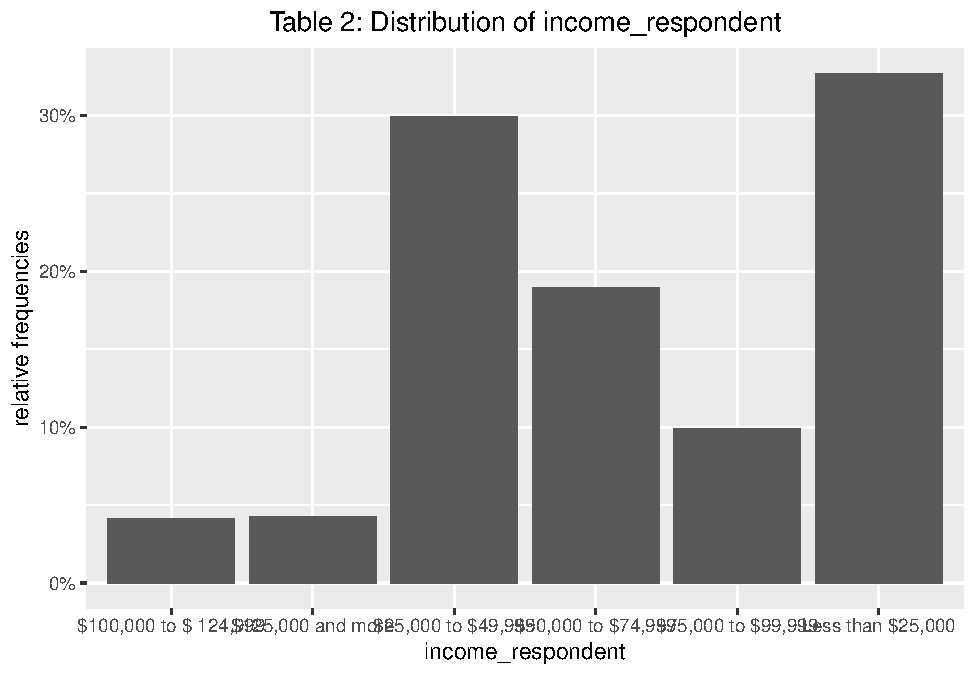
\includegraphics{ProblemSet2-template_files/figure-latex/unnamed-chunk-3-5.pdf}

\begin{verbatim}
## 
## Call:
## lm(formula = feelings_life ~ ., data = .)
## 
## Residuals:
##     Min      1Q  Median      3Q     Max 
## -8.5047 -0.6298  0.1827  1.2435  3.0573 
## 
## Coefficients:
##                          Estimate Std. Error t value Pr(>|t|)    
## (Intercept)               7.24976    0.03636 199.401  < 2e-16 ***
## is_marriedTRUE            0.58801    0.03036  19.368  < 2e-16 ***
## is_living_common_lawTRUE  0.44515    0.04282  10.395  < 2e-16 ***
## is_divorcedTRUE          -0.05497    0.04516  -1.217 0.223528    
## is_separatedTRUE         -0.42950    0.06805  -6.312 2.82e-10 ***
## is_widowedTRUE            0.18210    0.04448   4.094 4.25e-05 ***
## is_ownedTRUE              0.32393    0.02727  11.877  < 2e-16 ***
## is_rented_dkTRUE          0.08340    0.20003   0.417 0.676739    
## is_religionTRUE           0.22056    0.02859   7.714 1.28e-14 ***
## is_religion_dkTRUE        0.18735    0.13276   1.411 0.158196    
## is_25_49TRUE              0.12240    0.02854   4.288 1.81e-05 ***
## is_50_74TRUE              0.15949    0.03281   4.861 1.18e-06 ***
## is_75_99TRUE              0.22677    0.04115   5.511 3.62e-08 ***
## is_100_124TRUE            0.21438    0.05883   3.644 0.000269 ***
## is_125TRUE                0.37420    0.05819   6.430 1.30e-10 ***
## ---
## Signif. codes:  0 '***' 0.001 '**' 0.01 '*' 0.05 '.' 0.1 ' ' 1
## 
## Residual standard error: 1.589 on 20116 degrees of freedom
## Multiple R-squared:  0.06299,    Adjusted R-squared:  0.06234 
## F-statistic: 96.59 on 14 and 20116 DF,  p-value: < 2.2e-16
\end{verbatim}

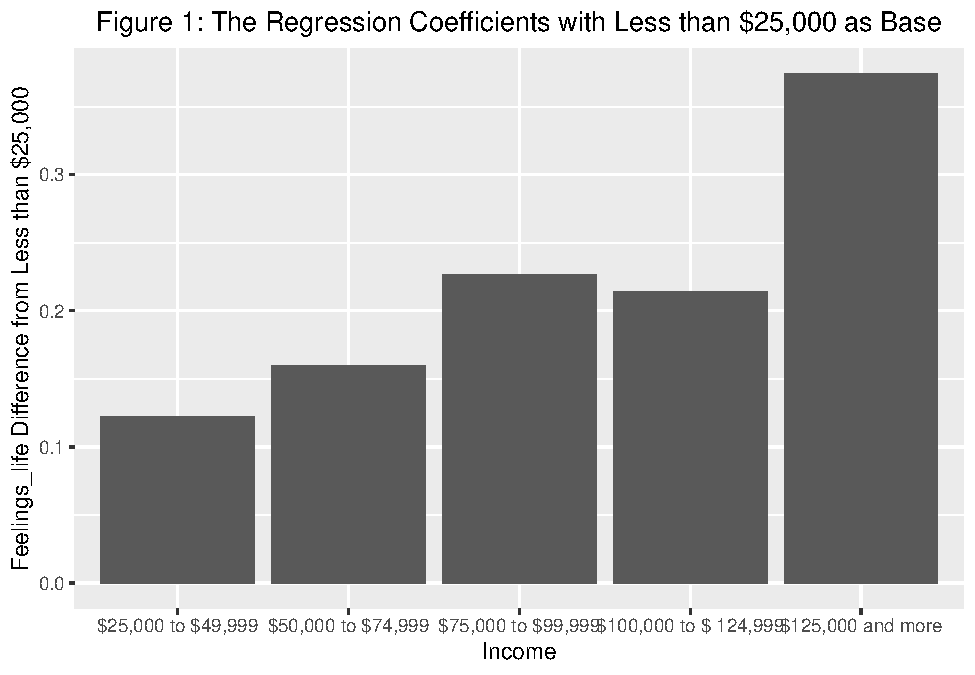
\includegraphics{ProblemSet2-template_files/figure-latex/unnamed-chunk-4-1.pdf}

\begin{verbatim}
## 
## Call:
## lm(formula = feelings_life ~ ., data = .)
## 
## Residuals:
##     Min      1Q  Median      3Q     Max 
## -8.5047 -0.6298  0.1827  1.2435  3.0573 
## 
## Coefficients:
##                          Estimate Std. Error t value Pr(>|t|)    
## (Intercept)               7.37216    0.03881 189.946  < 2e-16 ***
## is_marriedTRUE            0.58801    0.03036  19.368  < 2e-16 ***
## is_living_common_lawTRUE  0.44515    0.04282  10.395  < 2e-16 ***
## is_divorcedTRUE          -0.05497    0.04516  -1.217   0.2235    
## is_separatedTRUE         -0.42950    0.06805  -6.312 2.82e-10 ***
## is_widowedTRUE            0.18210    0.04448   4.094 4.25e-05 ***
## is_ownedTRUE              0.32393    0.02727  11.877  < 2e-16 ***
## is_rented_dkTRUE          0.08340    0.20003   0.417   0.6767    
## is_religionTRUE           0.22056    0.02859   7.714 1.28e-14 ***
## is_religion_dkTRUE        0.18735    0.13276   1.411   0.1582    
## is_0_25TRUE              -0.12240    0.02854  -4.288 1.81e-05 ***
## is_50_74TRUE              0.03710    0.03306   1.122   0.2618    
## is_75_99TRUE              0.10437    0.04133   2.526   0.0116 *  
## is_100_124TRUE            0.09199    0.05894   1.561   0.1186    
## is_125TRUE                0.25180    0.05823   4.325 1.54e-05 ***
## ---
## Signif. codes:  0 '***' 0.001 '**' 0.01 '*' 0.05 '.' 0.1 ' ' 1
## 
## Residual standard error: 1.589 on 20116 degrees of freedom
## Multiple R-squared:  0.06299,    Adjusted R-squared:  0.06234 
## F-statistic: 96.59 on 14 and 20116 DF,  p-value: < 2.2e-16
\end{verbatim}

\begin{verbatim}
## 
## Call:
## lm(formula = feelings_life ~ ., data = .)
## 
## Residuals:
##     Min      1Q  Median      3Q     Max 
## -8.5047 -0.6298  0.1827  1.2435  3.0573 
## 
## Coefficients:
##                          Estimate Std. Error t value Pr(>|t|)    
## (Intercept)               7.40925    0.04300 172.307  < 2e-16 ***
## is_marriedTRUE            0.58801    0.03036  19.368  < 2e-16 ***
## is_living_common_lawTRUE  0.44515    0.04282  10.395  < 2e-16 ***
## is_divorcedTRUE          -0.05497    0.04516  -1.217 0.223528    
## is_separatedTRUE         -0.42950    0.06805  -6.312 2.82e-10 ***
## is_widowedTRUE            0.18210    0.04448   4.094 4.25e-05 ***
## is_ownedTRUE              0.32393    0.02727  11.877  < 2e-16 ***
## is_rented_dkTRUE          0.08340    0.20003   0.417 0.676739    
## is_religionTRUE           0.22056    0.02859   7.714 1.28e-14 ***
## is_religion_dkTRUE        0.18735    0.13276   1.411 0.158196    
## is_0_25TRUE              -0.15949    0.03281  -4.861 1.18e-06 ***
## is_25_49TRUE             -0.03710    0.03306  -1.122 0.261840    
## is_75_99TRUE              0.06728    0.04388   1.533 0.125260    
## is_100_124TRUE            0.05489    0.06072   0.904 0.366044    
## is_125TRUE                0.21471    0.05998   3.580 0.000345 ***
## ---
## Signif. codes:  0 '***' 0.001 '**' 0.01 '*' 0.05 '.' 0.1 ' ' 1
## 
## Residual standard error: 1.589 on 20116 degrees of freedom
## Multiple R-squared:  0.06299,    Adjusted R-squared:  0.06234 
## F-statistic: 96.59 on 14 and 20116 DF,  p-value: < 2.2e-16
\end{verbatim}

\begin{verbatim}
## 
## Call:
## lm(formula = feelings_life ~ ., data = .)
## 
## Residuals:
##     Min      1Q  Median      3Q     Max 
## -8.5047 -0.6298  0.1827  1.2435  3.0573 
## 
## Coefficients:
##                          Estimate Std. Error t value Pr(>|t|)    
## (Intercept)               7.47653    0.04949 151.073  < 2e-16 ***
## is_marriedTRUE            0.58801    0.03036  19.368  < 2e-16 ***
## is_living_common_lawTRUE  0.44515    0.04282  10.395  < 2e-16 ***
## is_divorcedTRUE          -0.05497    0.04516  -1.217   0.2235    
## is_separatedTRUE         -0.42950    0.06805  -6.312 2.82e-10 ***
## is_widowedTRUE            0.18210    0.04448   4.094 4.25e-05 ***
## is_ownedTRUE              0.32393    0.02727  11.877  < 2e-16 ***
## is_rented_dkTRUE          0.08340    0.20003   0.417   0.6767    
## is_religionTRUE           0.22056    0.02859   7.714 1.28e-14 ***
## is_religion_dkTRUE        0.18735    0.13276   1.411   0.1582    
## is_0_25TRUE              -0.22677    0.04115  -5.511 3.62e-08 ***
## is_25_49TRUE             -0.10437    0.04133  -2.526   0.0116 *  
## is_50_74TRUE             -0.06728    0.04388  -1.533   0.1253    
## is_100_124TRUE           -0.01239    0.06543  -0.189   0.8499    
## is_125TRUE                0.14743    0.06473   2.278   0.0228 *  
## ---
## Signif. codes:  0 '***' 0.001 '**' 0.01 '*' 0.05 '.' 0.1 ' ' 1
## 
## Residual standard error: 1.589 on 20116 degrees of freedom
## Multiple R-squared:  0.06299,    Adjusted R-squared:  0.06234 
## F-statistic: 96.59 on 14 and 20116 DF,  p-value: < 2.2e-16
\end{verbatim}

\begin{verbatim}
## 
## Call:
## lm(formula = feelings_life ~ ., data = .)
## 
## Residuals:
##     Min      1Q  Median      3Q     Max 
## -8.5047 -0.6298  0.1827  1.2435  3.0573 
## 
## Coefficients:
##                          Estimate Std. Error t value Pr(>|t|)    
## (Intercept)               7.46414    0.06507 114.716  < 2e-16 ***
## is_marriedTRUE            0.58801    0.03036  19.368  < 2e-16 ***
## is_living_common_lawTRUE  0.44515    0.04282  10.395  < 2e-16 ***
## is_divorcedTRUE          -0.05497    0.04516  -1.217 0.223528    
## is_separatedTRUE         -0.42950    0.06805  -6.312 2.82e-10 ***
## is_widowedTRUE            0.18210    0.04448   4.094 4.25e-05 ***
## is_ownedTRUE              0.32393    0.02727  11.877  < 2e-16 ***
## is_rented_dkTRUE          0.08340    0.20003   0.417 0.676739    
## is_religionTRUE           0.22056    0.02859   7.714 1.28e-14 ***
## is_religion_dkTRUE        0.18735    0.13276   1.411 0.158196    
## is_0_25TRUE              -0.21438    0.05883  -3.644 0.000269 ***
## is_25_49TRUE             -0.09199    0.05894  -1.561 0.118626    
## is_50_74TRUE             -0.05489    0.06072  -0.904 0.366044    
## is_75_99TRUE              0.01239    0.06543   0.189 0.849850    
## is_125TRUE                0.15982    0.07710   2.073 0.038201 *  
## ---
## Signif. codes:  0 '***' 0.001 '**' 0.01 '*' 0.05 '.' 0.1 ' ' 1
## 
## Residual standard error: 1.589 on 20116 degrees of freedom
## Multiple R-squared:  0.06299,    Adjusted R-squared:  0.06234 
## F-statistic: 96.59 on 14 and 20116 DF,  p-value: < 2.2e-16
\end{verbatim}

\begin{verbatim}
## 
## Call:
## lm(formula = feelings_life ~ ., data = .)
## 
## Residuals:
##     Min      1Q  Median      3Q     Max 
## -8.5047 -0.6298  0.1827  1.2435  3.0573 
## 
## Coefficients:
##                          Estimate Std. Error t value Pr(>|t|)    
## (Intercept)               7.62396    0.06536 116.650  < 2e-16 ***
## is_marriedTRUE            0.58801    0.03036  19.368  < 2e-16 ***
## is_living_common_lawTRUE  0.44515    0.04282  10.395  < 2e-16 ***
## is_divorcedTRUE          -0.05497    0.04516  -1.217 0.223528    
## is_separatedTRUE         -0.42950    0.06805  -6.312 2.82e-10 ***
## is_widowedTRUE            0.18210    0.04448   4.094 4.25e-05 ***
## is_ownedTRUE              0.32393    0.02727  11.877  < 2e-16 ***
## is_rented_dkTRUE          0.08340    0.20003   0.417 0.676739    
## is_religionTRUE           0.22056    0.02859   7.714 1.28e-14 ***
## is_religion_dkTRUE        0.18735    0.13276   1.411 0.158196    
## is_0_25TRUE              -0.37420    0.05819  -6.430 1.30e-10 ***
## is_25_49TRUE             -0.25180    0.05823  -4.325 1.54e-05 ***
## is_50_74TRUE             -0.21471    0.05998  -3.580 0.000345 ***
## is_75_99TRUE             -0.14743    0.06473  -2.278 0.022755 *  
## is_100_124TRUE           -0.15982    0.07710  -2.073 0.038201 *  
## ---
## Signif. codes:  0 '***' 0.001 '**' 0.01 '*' 0.05 '.' 0.1 ' ' 1
## 
## Residual standard error: 1.589 on 20116 degrees of freedom
## Multiple R-squared:  0.06299,    Adjusted R-squared:  0.06234 
## F-statistic: 96.59 on 14 and 20116 DF,  p-value: < 2.2e-16
\end{verbatim}

For the marital statue, when setting is\_single as base, the other
levels except is\_divorcedTRUE are significant. is\_ownedTRUE is
significant and is\_religionTRUE are significant in each level. All the
levels of income are significant when setting the below 25 as base
level. But when looking into each of them, only the last level
is\_125TRUE will cause a large change. The bar plot also shows that the
feelings life increase slowly and has flutuation in the first four
level, only the last level has obvious change.

\hypertarget{discussion}{%
\subsection{Discussion}\label{discussion}}

In conclusion, the marital statue, house owning or renting, religion and
income are all significant factors that will affect the feelings of
life. For marital statues, getting married and living together do have a
more satisfied life than singles, while divorced and seperate has a less
satified life than single. Interestingly, widowed seems more satified,
and the divorced in not significant. For own\_rent, people owning a
house will be more satified than those without living place, while
renting is unsignificance. For religion, having a belief will be more
satisfied than those without belief. And for income, all the level
showed its significance, the feeling of life seems to increase as the
income level increase. However, when looking into each level precisely,
we find out that each levle show significance compared to below 25
level, and the above 125 level show significance to each level below.
However, for the middle four levels between the highest and lowest, the
increase is not that significant, even it appears fluctuation. The plot
also shows a similiar result, such that the lowest level is obvious low
and the highest level is obvious high, while the middle of them increase
slowly.

\hypertarget{weaknesses}{%
\section{Weaknesses}\label{weaknesses}}

The linear model itself may be not precise enough. Though the study of
life feeling and income is fine, but other factors are difficult to
judge.

\hypertarget{next-steps}{%
\section{Next Steps}\label{next-steps}}

For the next step, I may learn some interesting finding in this study,
such as the is\_widowedTRUE level in marital variable. Also, I would
continue to study if there is a better statistic model for the data.

\hypertarget{references}{%
\subsection{References}\label{references}}

{[}1{]} Wickham et al., (2019). Welcome to the tidyverse. Journal of
Open Source Software, 4(43), 1686,
\url{https://doi.org/10.21105/joss.01686}

{[}2{]} Kirill Müller (2017). here: A Simpler Way to Find Your Files. R
package version 0.1. \url{https://CRAN.R-project.org/package=here}

{[}3{]} gss csv

\end{document}
